


\section{Dogma central de la biología molecular}

\begin{figure}[H]
    \centering
    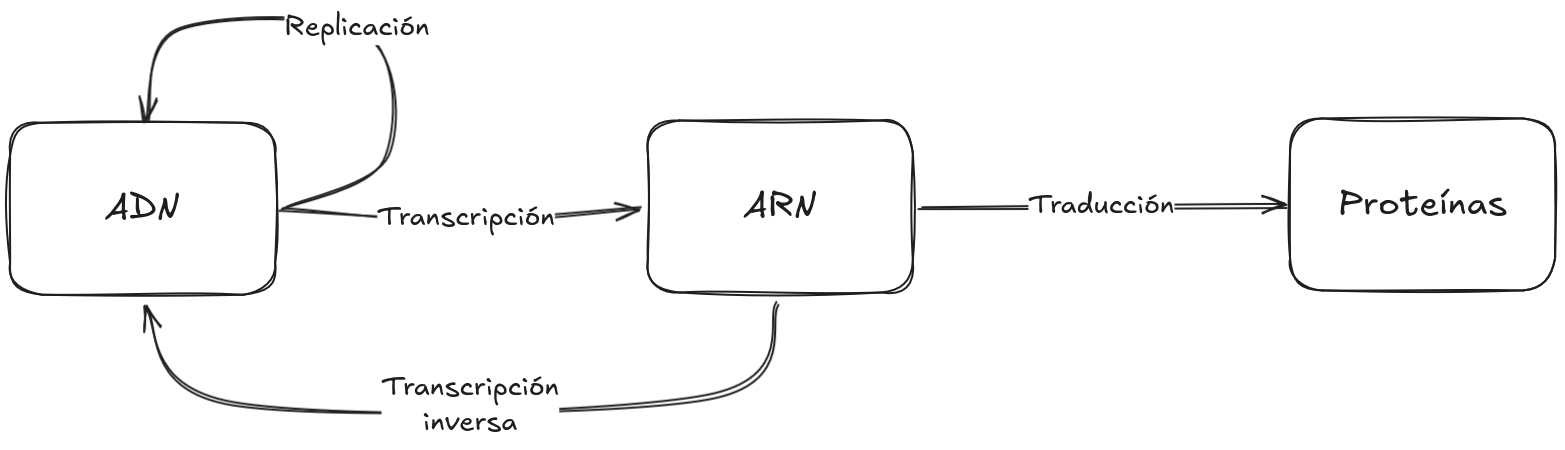
\includegraphics[width=0.85\linewidth]{./images/dogma_central.png}
    \caption{Dogma central de la biología}
    \label{fig:dogma_central}
\end{figure}



\section{Exones e intrones}



\section{Transcripción del ADN}

La transcripción del ADN es un proceso celular el cual consiste en la síntesis de ARN a partir de un molde de ADN. Este ARN resultante obtiene el nombre de transcrito.

Este ARN resultante puede ser de varios tipos, pero podemos diferenciar 2 grandes tipos: el ARN informativo (principalmente ARN mensajero (ARNm)) y el ARN funcional.

El ARN informativo tiene la función de ser convertido a proteínas en un proceso llamado traducción, el cual se verá más adelante. Por otro lado, el ARN funcional consiste en todo aquel ARN que no se traduce a proteínas, sino que tiene otra función o actividad dentro la célula. A lo largo de esta sección se estudiarán los ARN funcionales, los cuales se enlistan a continuación:

\begin{itemize}
    \item ARN ribosomal (ARNr)
    \item ARN de transferencia (ARNt)
    \item Micro ARN's
	    \begin{itemize}
	        \item ARNnp (ARN nucleares pequeños): Interacciónan con proteínas formando los complejos de ribonucleotproteínas
	        \item ARNcp (ARN citoplasmáticos pequeños): Intervienen en el transporte de los polipéptidos
	    \end{itemize}
\end{itemize}

\subsection{ARN ribosomal (ARNr)}

La función de los ARNr es formar ribosomas que luego estarán encargados de la síntesis de proteínas.

\subsection{Síntesis de ARNr en bacterias}

Partes del gen codificante: Los ARNr (ARN ribosomal) se procesan a partir de zonas específicas de ADN, las cuales cuentan la característica de estar formada por las siguientes partes:

\begin{itemize}
    \item Promotor: Es la linea de ADN que indica dónde inicia la zona que codifica ARNr.
    \item Gen de ARNr: Es la linea que luego se convertirá en ARNr.
    \item Terminador: Es una linea de ADN que indica dónde termina la zona que codifica ARNr.
\end{itemize}

\subsection{Enzimas encargadas del corte}

Existen 3 enzimas que se encargan de "cortar" la linea codificante: La endonucleasa, la ARNasa III y la ARNasaM

\begin{itemize}
    \item Endonucleasa y ARNasa III: Se encargan de cortar el gen de ARNr ya liberado del promotor y del terminador.
    \item ARNasa M: Se encarga de separar, en caso de existir, la p16s de de algún ARNt que pueda venir también codificado en la cadena de ADN.
\end{itemize}

\subsection{Estructura de los ribosomas de procariotas}

Los ribosomas ya formados tienen un tamaño de 70s\footnote{s = unidad de sedimentación} . Este valor es dado a partir de su nivel de sedimentación.
Estos ribosomas formados con los ARNr se dividen en subunidades, una mayor y una menor, las cuales tienen algunas diferencias:

\begin{itemize}
    \item Subunidad mayor (50s): Se conforma de los siguientes ARNr, a los cuales se le añaden alrededor de 34 proteínas extra.
        \begin{itemize}
            \item p23s
            \item p5s
        \end{itemize}
    
    \item Subunidad menor (30s): Se conforma del ARNr p16s, y a este ARNr se le añaden alrededor de 21 proteínas extra. 
\end{itemize}

\subsection{Síntesis de ARNr en eucariotas}

Partes del gen codificante: Los ARNr (ARN ribosomal) se procesan a partir de zonas específicas de ADN, las cuales cuentan la característica de estar formada por las siguientes partes:

\begin{itemize}
    \item Promotor: Es la linea de ADN que indica dónde inicia la zona que codifica ARNr.
    \item Gen de ARNr: Es la linea que luego se convertirá en ARNr.
    \item Secuencias espaciadoras: Se separan los genes de diferentes ARNr's con secuencias espaciadoras.
    \item Terminador: Es una linea de ADN que indica dónde termina la zona que codifica ARNr.
\end{itemize}

\subsection{Proteínas involucradas en la síntesis}

Durante la síntesis del ARNr en eucariotas no solo se transcriben los genes, sino que también se usa el apoyo de proteínas provenientes del citosol para el ensamblaje de los ribosomas. (RTL y RPS)

\subsection{Estructura de los ribosomas de eucariotas}

Los ribosomas ya formados tienen un tamaño de 80s\footnote{s = unidad de sedimentación} . Este valor es dado a partir de su nivel de sedimentación.
Estos ribosomas formados con los ARNr se dividen en subunidades, una mayor y una menor, las cuales tienen algunas diferencias:

\begin{itemize}
    \item Subunidad mayor (60s): Se conforma de los siguientes ARNr, a los cuales se le añaden alrededor de 49 proteínas extra.:
        \begin{itemize}
            \item p28s
            \item p5.8s
            \item p5s: Este, a diferencia de las anteriores, viene del nucleo. 
        \end{itemize} 
        
    \item Subunidad menor (40s): Se conforma del ARNr p18s, y a este ARNr se le añaden alrededor de 33 proteínas extra.
\end{itemize}

\subsection{ARN de transferencia (ARNt)}

El ARN de transferencia cumple la función de transportar aminoácidos para la síntesis de proteínas. Su estructura se compone de las siguientes partes:

\begin{itemize}
    \item Asa aceptor: Extremo del tallo que lleva el aminoácido 
    \item Asa TYC: Contiene una secuencia de bases de timina y pseudouridina y es crucial ara la interacción de la molécula con el ribosoma.
    \item Asa D: Recibe su nombre por la presencia de una base nitrogenada modificada (dihidrouridina), y es importante para el reconocimiento por parte de las enzimas aminoacil-ARNt sintetasa que une el aminoácido correcto al ARNt.
    \item Anticodón: Zona complementaria a un codón específico del ARNm
    \item Unión aminoácido-ARNt: La unión entre un aminoácido y un ARNt se da gracias a enzimas llamadas aminoacil-ARNt sintetasa, las cuales son cruciales para la síntesis de proteínas que unen de forma covalente un aminoácido a su molécula de ARNt correspondiente. A esto se le llama "carga del ARNt".
\end{itemize}

\section{Moléculas de ARN informativas}

Estas son las moléculas que si se van a traducir posteriormente a proteínas, y principalmente hablamos del ARNm.

En bacterias el tanscrito primario, tal y como se sintetisa, ya es el ARNm maduro listo para sintetizar proteínas. Existe solo 1 ARNpol. La ARNpol es una holoenzima requiere de un factor sigma ($\sigma$) para formarse y llevar a cabo sus funciones. Se compone de subunidades $\alpha , \beta , \beta ' , \sigma , \omega$. Transforma la timina a uracilo. Con frecuencia los ARN son poligénicos o policistrónicos, de manera que un solo ARNm contiene información para la síntesis de varios polipétptidos distintos.

Existen 3 ARNpol, cada una con diferente función:

\begin{enumerate}
    \item Sintesis de precursores de ARNr
    \item Produce ARNhn y ARNm
    \item Transcribe los precursores de las ARN (t, np, cp). Transcribe también los genes para el ARN 5 que forma parte de la subunidad grande de los ribosonas
\end{enumerate}

En eucariotas el ARN recién transcrito se denomina ARNhn (heterogéneo nuclear), y es un "pre-ARNm" que es procesado antes de convertirse en un ARNm maduro. En las eucariotas los ARNm son monosistronicos, quiere decir, cada gen corresponde a una única proteína.
	
\section{Transcripción del ADN en eucariotas}

La transcrición de ADN en eucariotas cuenta con 3 fases:

\begin{enumerate}
    \item Iniciación: Identifica inicio de Unidad Transcripcional, luego se define el sentido de la transcripción. Para este paso son esenciales las regiones promotoras (promotor).
    \item Elongación: Una vez dado el primer enlace fosfodiester, se considera que inició la elongación, proceso en elcual la ARNpol avanza por el gen codificante generando ARN.
    \item Terminación: Una vez llegado al final del gen codificante, se vuelve a doblar el ADN, esto puede pasar mediante 2 mecanismos:
        \begin{itemize}
            \item Dependiente de $\rho$
            \item Independiente de $\rho$
        \end{itemize}
\end{enumerate}

\subsection{Regiones promotoras}

\begin{itemize}
    \item +1 (CAT): Inicia siempre en A o G
    \item -10 (TATA box): Se compone de la secuencia de bases (TATAAT): También se conoce como la Caja de Pribnow
    \item -35 (TTGACAT): En estas secuencias promotoras se une un factor llamado factor sigma ($\sigma$). De este existen distintos tipos:
    \item 70: Busca en las secuencias -35 y -10
    \item 32: Generalmente actua en genes de choque térmico
    \item 54: Para iniciar la transcripción se necesita separar las hebras de ADN, y tal separación se da en la región -10, la cual tiene una alta concentración de bases T y G.
\end{itemize}

\subsection{Partes de la ARNpol}

La ARNpol de las células procariotas se compone de 5 subunidades ($2 \ \alpha, \beta , \beta ', \omega$) y un cofactor sigma ($\sigma$).

La subunidad $\alpha$ cuenta con una función principalmente estructural. También inician la cadena con ayuda de promotores. Secuencias reguladoras.

La subunidad $\beta$ es la que tiene actividad polimerasa y cataliza la síntesis de ARN. Enlace fosfodiester, transcribe de 5' a 3'.

La subunidad $\beta '$ es la subunidad que se une a la hebra no codificante. Secuencia molde de ADN, no codificante.

El cofactor $\sigma$: se separa despues de 10 a 15 nucleótidos mientras que la ARN-polimerasa continua. El factor sigma, despues de separarse, busca nuevos promomotores para iniciar una nueva transcripción.

Existe también la subunidad $\omega$.

\subsection{Terminación independiende de $\rho$}

Para esta terminación existen regiones del ADN llamadas regiones palindromicas (como palíndromos), las cuales son ricas en guanincas y citosinas (GC) y precede a otra zona rica en adenintas y timinas (AT).
Una vez se llega a esta zona, el transcrito forma una estructura en horquilla con una cola rica en uracilos (U), lo que induce que se termine la transcripción y todas las pertes involucradas se separen.

\subsection{Terminación dependiende de $\rho$}

Para zonas donde no existen regiones palindrómicas existe el factor rho ($\rho$), el cual cuenta con una estructura hexamérica y presenta actividad ATPasa.
Este factor se une a región que consta de una secuencia de 72 nucleótidos y debilita la interacción molde-transcrito, haciendo que se separen y que, por ende, se termine la transcripción.

\section{Splicing alternativo}

En diferentes tejidos de un mismo individuo o en el mismo tejido en diferentes momentos del desarrollo se pueden producir procesamientos distintos del mismo ARNhn. Como consecuencia, en cada tejido o momento del desarrollo se produce un ARNm maduro diferente que da lugar a una proteína (polipéptido distinto.)

\begin{figure}[H]
    \centering
    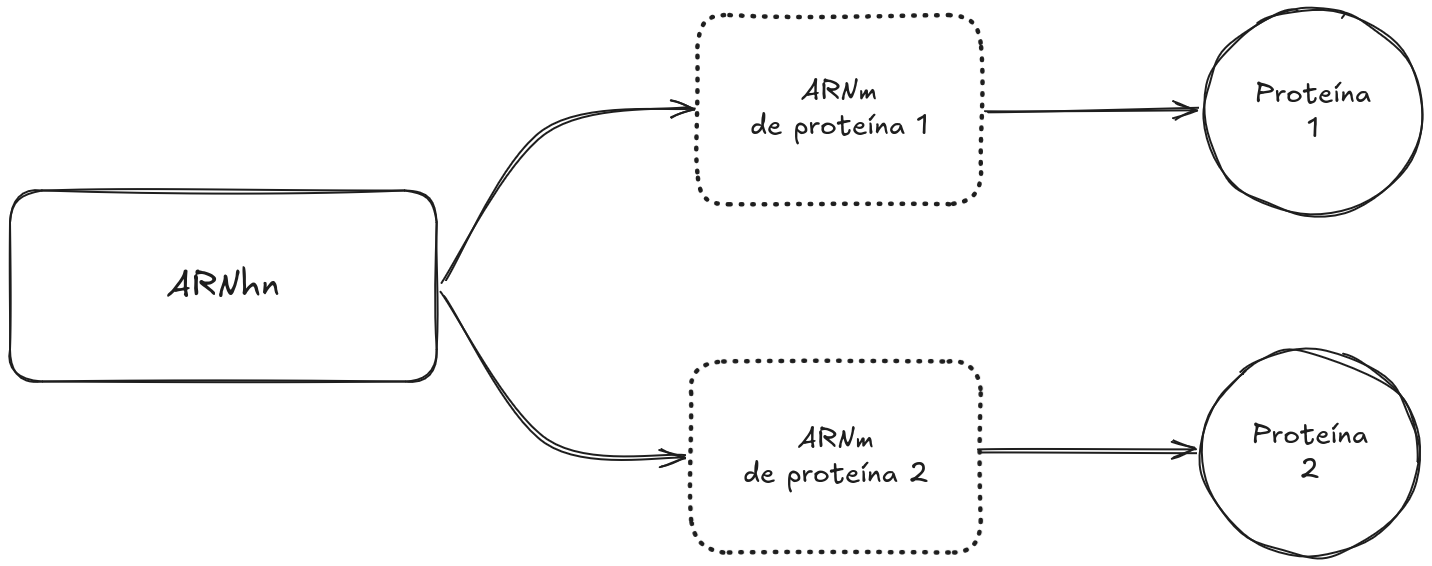
\includegraphics[width=0.85\linewidth]{./images/splicing_alternativo.png} 
    \caption{Splicing alternativo}
    \label{fig:splicing_alt}
\end{figure}

Un ejemplo de procesamiento alternativo es lo que sucede en la tiroides e hipotálamo, en los que el mismo ARNhn da lugar, con procesamientos diferentes, da lugar al péptido de calcitonina en la tiroides y al péptido CGRP en el hipotálamo.

\section{Procesamiento del ARN}



\section{Modificaciones post-transcripcionales y co-transcripcionales}



\section{Síntesis de proteínas (traducción)}



